\scanpage{112}
\mspage{\deleted{\unsure{55|56}}}

\[
t_0=\rho s_0 \tag*{(33)}
\]

\figure{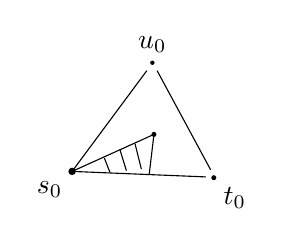
\begin{tikzpicture}[x=1cm,y=1cm,baseline]
\coordinate (s) at (0,0); \coordinate (t) at (1.8,-.08); \coordinate (u) at (1.02,1.38);
\draw (s)--(.95,1.28) (1.08,1.28)--(1.76,.02) (1.7,-.07)--(s);
\draw (s)--(1.04,.47)--(.98,-.035);
\draw (.41,.17)--(.48,-.01) (.61,.27)--(.69,.01) (.8,.35)--(.88,.03);
\fill (s) circle (.047) (t) circle (.032) (u) circle (.028) (1.04,.47) circle (.032);
\node[below left] at (s) {$s_0$}; \node[below right] at (t) {$t_0$}; \node[above] at (u) {$u_0$};
\end{tikzpicture}}

(p.ex. $\rho={}$``rotation d'un cran autour de $u_0$, de $s_0$ vers $t_0$''), on aura

% slanted
\margin{plus \unsure{joliment} : $\rho=\rho_1={}$ symétrie p.r. au centre de l'arête $\{s_0,t_0\}$, p. ex., ou $\rho=\rho_\infty$ (rotation de \unsure{un|$-1$} tiers de tour autour du centre de la face $\{s_0,t_0,u_0\}$\unsure{)}}

\[
\lambda^{-1}t_0=\lambda^{-1}\rho s_0=\rho\lambda^{-1}s_0
\]

posons

\[
\left.\begin{aligned}\lambda^{\deleted{\unsure{-1|1}}}s_0&=g.s_0\\
\lambda^{-1}s_0&=g^{-1}.s_0\end{aligned}\quad\right|\quad
\text{où }g\in\operatorname{Norm}_{G_0^+}(G^+_{0\,s_0})
\]

la relation (32 bis) s'écrit aussi

\[
\{g.s_0,\rho g^{-1}\deleted{\unsure{t}}s_0\}\in A_0
\]

ou encore

\[
\exists u\in G_0^+,\quad\text{avec }\ u(s_0,t_0)=(gs_0,\rho g^{-1}t_0)
\]

ou encore, écrivant $t_0=\rho s_0$

\[
u.s_0=g.s_0 \qquad u\rho.s_0=\rho g^{-1}.\deleted{\unsure{t}}s_0
\]

soit encore

\[
g^{-1}u\in G^+_{0\,s_0},g(\underbrace{\rho^{-1}u\rho})\in G^+_{0\,s_0}
\]

donc l'axiome $\mathrm T_0\,3$ équivaut :

% slanted
\margin{on a posé $g^{-1}u=z$ i.e. $u=gz$}

\[
\begin{aligned}
(\mathrm T_0\,3')\quad &\forall g\in\operatorname{Norm}_{G_0^+}(G^+_{0\,s_0}),\ \exists z\in G^+_{0\,s_0}\quad\text{(néc$^{\rm t}$ unique!)}\\
&\text{tel qu'on ait}\\
&g.\deleted{\unsure{\rho^{-1}|\rho}}\operatorname{int}(\rho^{-1})(gz)\in G^+_{0\,s_0}
\end{aligned}\tag*{(34)}
\]

% slanted
\margin{où $\rho$ est \deleted{\unsure{l'unique|l'antique}} \inserted{un} élément de $G_0^+$ fixé \deleted{\unsure{une}} fois pour toutes, tel que $\rho s_0=t_0$, NB \unsure{la|$\rho$}, $\rho=\rho_1$ ou $\rho=\rho_\infty$}

Si on se rappelle que la situation d'un 2-polyèdre orienté \inserted{triangulé} régulier \deleted{\unsure{avec|com.|comme}}, spécifié par $(s_0,t_0,u_0)$, équivaut : celle du groupe $G_0^+$, avec des
% archive sheet number: 111
